\documentclass{beamer}
\usetheme{ConnectivityLab}
\usepackage{times}
\usepackage{graphicx}
\usepackage{verbatim}
\usepackage{outlines}
\usepackage{fancyhdr}
\usepackage{subfigure}
\usepackage{cancel}
\usepackage{bibentry}
\usepackage{varwidth}
\usepackage{etoolbox}
\usepackage{epstopdf}
%%%%%%%%%%%%%%%%%%%%%%%%%%%%%%%%%%%%%%%%%%%%%%%%%%%%%%
%%%%%%%%%%%%%%%%%%%%%%%%%%%%%%%%%%%%%%%%%%%%%%%%%%%%%%

\title {
    Progress report
}
\author {
    Yin-Hong, Hsu
}
\date {
    02 07, 2017
}

%%%%%%%%%%%%%%%%%%%%%%%%%%%%%%%%%%%%%%%%%%%%%%%%%%%%%%
%%%%%%%%%%%%%%%%%%%%%%%%%%%%%%%%%%%%%%%%%%%%%%%%%%%%%%

\begin{document}
\begin{frame}
    \titlepage
\end{frame}

%%%%%%%%%%%%%%%%%%%%%%%%%%%%%%%%%%%%%%%%%%%%%%%%%%%%%%
%%%%%%%%%%%%%%%%%%%%%%%%%%%%%%%%%%%%%%%%%%%%%%%%%%%%%%

\begin{frame}{Outline}
    \tableofcontentsgather
    \tableofcontents
\end{frame}

%%%%%%%%%%%%%%%%%%%%%%%%%%%%%%%%%%%%%%%%%%%%%%%%%%%%%%
%%%%%%%%%%%%%%%%%%%%%%%%%%%%%%%%%%%%%%%%%%%%%%%%%%%%%%

\section{Survey of RAP in NB-IoT and LTE}

\begin{frame}{Aim}
    \begin{itemize}
        \item {Migrate the background of system to NB-IoT}
    \end{itemize}
\end{frame}

\begin{frame}{Term}
    \begin{itemize}
        \item {AC - Access Class 0-9 for general, 11-15 for certain device}
        \item {CE level - Coverage Enhancement (0-2 to against different signal fading)}
    \end{itemize}
\end{frame}

\begin{frame}{NB-IoT v.s. LTE (same)}
    \begin{itemize}
        \item {They got same message flow}
        \item {They use ACB on congestion control}
    \end{itemize}
\end{frame}

\begin{frame} {RAP message flow} 
    \begin{figure}[t]
    \centering
    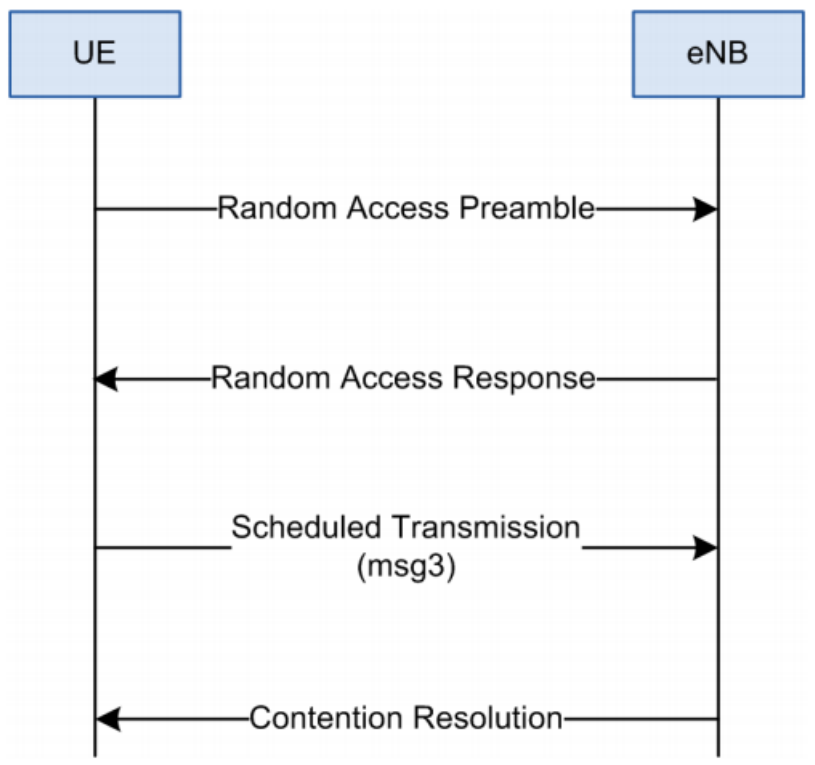
\includegraphics[width=0.7\textwidth]{figures/rapFlow.png}
    \setbeamerfont{caption}{size=\tiny}
\end{figure}

\begin{frame}{NB-IoT v.s. LTE (different)}
    \begin{itemize}
        \item {NB-IoT have different maximum retransmit time and frequency according to each CE level}
        \item {In NB-IoT congestion control, UEs with AC 0-9 use EAB and AC 11-15 use ACB}
        \item {In NB-IoT, it use SIB-NB to deliver system information instead of traditional SIB}
    \end{itemize}
\end{frame}

\begin{frame} {RAP for NB-IoT} 
    \begin{figure}[t]
    \centering
    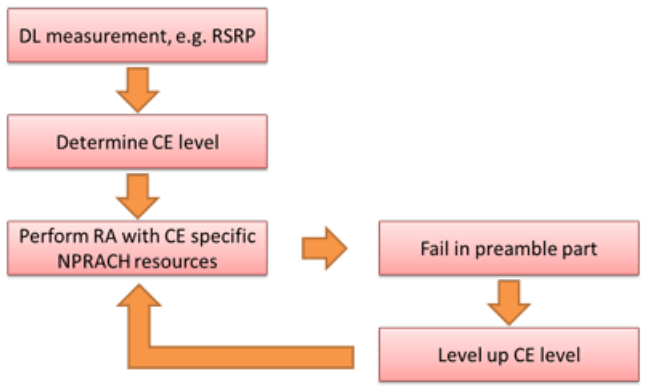
\includegraphics[width=0.7\textwidth]{figures/rapInNB.png}
    \setbeamerfont{caption}{size=\tiny}
    \caption{get post data by http}
\end{figure}

%%%%%%%%%%%%%%%%%%%%%%%%%%%%%%%%%%%%%%%%%%%%%%%%%%%%%%
%%%%%%%%%%%%%%%%%%%%%%%%%%%%%%%%%%%%%%%%%%%%%%%%%%%%%%
\section{}

\begin{frame}
    \centering
    \Large{Thanks for Your Attentions}
\end{frame}

\end{document}
